\documentclass[thesis.tex]{subfiles}
\begin{document}

\chapter{Introduction}
\label{chap:introduction}

% An image right here at the top can look really cool!

\section{Introduction}
The current internet  has exceeded any expectations. The engineers creating it in the 1960 couldn't even imagine the impact and various use of their creation. Only few user participated in the early internet without considering security and protection against attacks as a key aspect. There were so few people that they knew who they can trust and who not.

Today there are billions of user and billions of devices connected to each other \todo{Source for this}. There are malicious user trying to steal account information or fiends who overload resources and disrupt services. More and more services are created each year running on the internet and trying to provide a service to user. Each company has to know the newest security risks and attack types to be competitive and trustworthy. 

There are many types of problems with the current internet protocols. There are far more fixes and solutions with them, but each of them has to be accepted by the majority of the users and supported by the network device manufacturers. The acceptance of IPv6, a protocol released in 1996, is in 2017 low but the internet ran out of Ipv4 addresses years ago. \todo{More accurate numbers/dates!}.

Instead of fixing the current internet and having a brown field situation there are also people creating a better green field solution. They want to solve the problems without limitations of the current protocols and their implicit fundamental problems. One of the solutions is \textbf{SCION}, an acronym for \textbf{S}calability, \textbf{C}ontrol and \textbf{I}solation \textbf{O}n next-generation \textbf{N}etworks, which will be explained in detail in \autoref{chap:basics}.


\section{Motivation}
One of the many problems described previously is the strong increase of data usage on the internet. The DE-CIX in Frankfurt, Germany, a data carrier, registers with each year an higher amount of data. The graph in \autoref{fig:intro:decixData} shows this increase . In 2014 the highest registered bits per second was around three tera bytes / s. Three years later in 2017 the peak was at 6 tera byte, twice the amount. 

In the advent of video streaming in form of Video on Demand (VOD) via services like Youtube and Netflix and live video streaming like Twitch the data usage of the users increased rapidly. There is also an increasing demand for higher resolutions, which results in bigger video sizes. The current standard of Full HD for a video will be succeeded by new standards like the 4k. The user also demands for a higher refresh rate. Currently the videos are sent with 30fps, but there is a benefit sing 60fps or even 144fps for real fast movements.

But videos are not the only reason for a higher bandwidth usage. Big Data companies processing petabytes of data each day rely on a stable and high bandwidth connection. There is also a trend with Internet-of-Things (IoT) to install small devices which collect and send data through the internet.

\begin{figure}
    \centering
    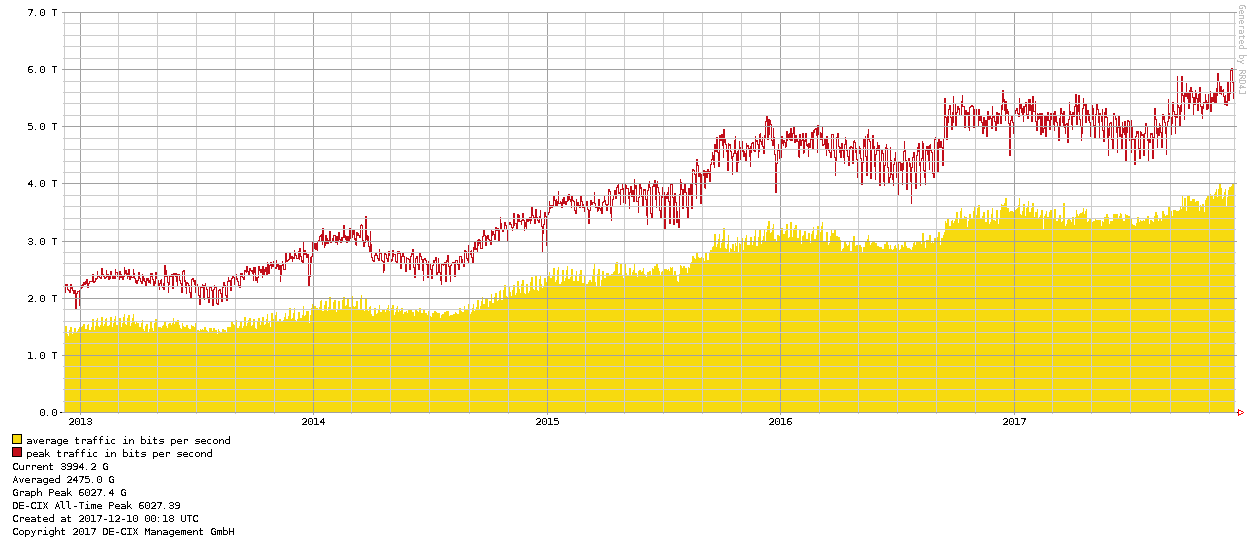
\includegraphics[width=0.95\linewidth]{20171210_1515_decix_data}
    \caption*{\tiny{ \url{https://www.de-cix.net/en/locations/germany/frankfurt/statistics} (10.12.2017)}}
    \label{fig:intro:decixData}
    \caption{5 year statistics of DE-CIX traffic}
\end{figure}

\todo{Add picture of DE-CIX current bandwidth}

One solution to solve this problems is to scale-up and install more and more bandwidth capacities like fiber cables or newer devices. This is inefficient and consumes probably more energy and increases so the running costs. There are also physical limits for improving the performance so that a small benefit results in high costs.

Another solution is to better utilize the current resources as it is done with the multi path process in SCION. The user can split their data and sent the packets via multiple connections. This leads to a better usage of the available bandwidth in the network. In currents internet this is not possible, because the router are deciding for themselves which route to take to the destination. 

\begin{figure}[h]
    \centering
    \begin{tikzpicture}
    \node[shape=rectangle,draw=black] (1-1) at (0,0) {1-1};
    \node[shape=rectangle,draw=black] (1-2) at (2,-1) {1-2};
    \node[shape=rectangle,draw=black] (1-3) at (2,1) {1-3};
    \node[shape=rectangle,draw=black] (1-4) at (4,0) {1-4};
    
    \path[-]	
    (1-1) edge node[sloped, anchor=center, below] {\tiny 1GB/s} (1-2) 
    (1-1) edge node[sloped, anchor=center, above] {\tiny 1GB/s} (1-3)
    (1-1) edge node[sloped, anchor=center, above] {\tiny 1GB/s} (1-4)
    (1-2) edge node[sloped, anchor=center, below] {\tiny 1GB/s} (1-4)
    (1-3) edge node[sloped, anchor=center, above] {\tiny 1GB/s} (1-4)
    ;
    \path[-{Latex[width=3mm]}, dashed]
    (1-1) edge[bend right=10] (1-4)
    (1-1) edge[bend left=80] (1-4)
    (1-1) edge[bend right=80] (1-4)
    ;
    \end{tikzpicture}
    \caption{Example topology for multipath}
    \label{fig:intro:exampleMultipath}
\end{figure}


This new method shall encourages user to better utilize the network, but it can also be misused. In \autoref{fig:intro:exampleMultipath} is an example visualized. Each AS is connected with each other via a 1 gigabit/s connection. AS 1-1 can send AS 1-4 using single path data with a 1 gigabit/s directly. It could also uses the paths 1-1$\rightarrow$1-2$\rightarrow$1-4 and 1-1$\rightarrow$1-3$\rightarrow$1-4 to sends its data and increase its bandwidth to ideally 3 gigabit/s, if there is zero delay on the hops. This possibility rises the questions how to monitor and enforce the bandwidth usage of a one particular AS. When using a single path connection the measurement point is at the destination. If this AS exceeds its limit the destination router can drop packets. This solution is not possible in a multi path communication. It is important to find an answer for this question to avoid misuse.

\begin{easylist}
    \MyListProperties
    # Resources in networks (bandwidth, CPU time and memory usage)
    # Expected growth of bandwidth (D.IX? in Frankfurt) -> Importance of fair system
    #\todo{Source from Hausheer inauguration speech}
    ## \textit{Figure of growth}
    ## \textit{Figure of expected bandwidth usage in a few years}
    ## Source for currently unused bandwidth (if there is some source)
    # Multi-Path in SCION as a solution for bandwidth usage
    # Problem with a greedy user can cause (congestions)
\end{easylist}

\section{Goals} \label{bib:goals}
     \begin{easylist}
        \MyListProperties        
        # The thesis' main goal is to achieve a fair usage of bandwidth at multi-path communication in SCIONLab. The proposed solution must not use more resources (computation time, bandwidth) as it will gains through using the bandwidth more efficiently. A solution with a 100\% accuracy is useless if it uses too much resources. Because of this, the goals must be always reach a trade-off between efficiency (resource usage) and effects (resource gain).        
        # The first goal to verify is, that the proposed solution has to detect a greedy user at least at 85\% with a minimal performance impact of 5\%.         
        # The solution must also provide parameters to increase the accuracy of the detection rate, even when the performance impact will be higher. This is important for an adaption in systems who requires an higher detection.
        # It is also a goal to create a scalable solution working with topologies with up to 100 ASes. This goal will be achieved by minimizing the impact on network traffic for necessary protocols.        
        # The solution must be general enough for other network types with multi-path capability.        
        # Based on the previous goal, this thesis has to provide an implementation for SCION which can be merged and used inside SCIONLab.
        # It is not a goal to clarify whether a punishment can be legally enforced or not. This thesis will only provide a mechanism to identify and punish a greedy user, but does not worry about if this will violates a contract between an user and its internet provider.
    \end{easylist}

\section{Main Contribution}
    \begin{easylist}
        \MyListProperties
        # SpeedCam approach
        ## Measuring the used bandwidth
        ### Use a probabilistic approach 
        ## Regulate  / Punish greedy user
        
        # Implementation in SCIONLab
        ## Also usable in SCION
        ## Also usable in other networks
        ### Examples: Intranets 
    \end{easylist}
\section{Thesis Outline}
Describe the structure of this document.

Next chapter ....
\\
\autoref{chap:prevwork} discusses ...
\\
Our own contribution ... described in \autoref{chap:basics}.
Results are evaluated and discussed in \autoref{chap:eva}.
\\
Finally, \autoref{chap:concl} will summarize the thesis and give an outlook to possible future work.

\subfilebib % Makes bibliography available when compiling as subfile
\end{document}